\documentclass[pdftex,letterpaper,11pt]{article}%
\usepackage[export]{adjustbox}
\usepackage{multirow}
\usepackage[arabicsections]{dpugatex}
%\usepackage{dpppl}
%\usepackage{lscape}
\usepackage{pdflscape}

\usepackage{tikz}

\usepackage[british]{babel}
\usepackage{amssymb,amsmath,warpcol,url,ctable,multirow,caption,threeparttable,float,soul,gensymb}
%\usepackage[noend]{algpseudocode}
\makeatletter
\def\BState{\State\hskip-\ALG@thistlm}
\makeatother


\usepackage{subcaption}


\usepackage{xcolor,colortbl}
\definecolor{verylightgray}{gray}{0.90}
\newcommand{\verylightgray}[1]{\cellcolor{verylightgray}#1}


\usepackage{arydshln}
\setlength\dashlinedash{1.5pt}
\setlength\dashlinegap{2.5pt}
\setlength\arrayrulewidth{0.8pt}

\usepackage[utf8]{inputenc}
\usepackage{eurosym}
\usepackage{soul}
\setstcolor{red}
\definecolor{lightgreen}{rgb}{0.564706,0.933333,0.564706}
\soulregister\citet7 % These \soulregister commands allow us to avoid problems between soul functions (\hl, \st, ...) and these other functions (\citet,\citep,\ref,\footnote, ...). Include more if it is necessary.
\soulregister\citep7
\soulregister\cite7
\soulregister\ref7
\soulregister\footnote7
\soulregister\textit7
\soulregister\textbf7
\soulregister\textsc7
\soulregister\`7
\soulregister\'7
\soulregister\% 7
\usepackage{tabularx,tabulary}
\usepackage[osf]{mathpazo}
\usepackage[abs]{overpic}

\usepackage{hyperref}
\definecolor{darkblue}{rgb}{0.0,0.0,0.3}
\hypersetup{colorlinks=true, breaklinks=true, citecolor= darkblue, linkcolor=blue, urlcolor=blue}

\usepackage{chngcntr}

\newcommand{\mc}[3]{\multicolumn{#1}{#2}{#3}}
\newcommand{\mcc}[1]{\multicolumn{1}{c}{#1}}
\newcommand{\mcb}[1]{\multicolumn{1}{c}{\bf #1}}

\newcommand{\mr}[3]{\multirow{#1}{#2}{#3}}
\newcommand{\mg}[3]{\multicolumn{#1}{#2}{\verylightgray #3}}


\onehalfspacing%
%\doublespacing%

\newenvironment{tablenote}[1]{\begin{list}{}{\vskip-5mm\relax
\setlength{\leftmargin}{#1} \setlength{\rightmargin}{\leftmargin}}
\item[]\footnotesize\vskip-7pt
{\em Notes}:\space\ignorespaces}{\end{list}}

\newcommand{\jdlradded}[1]{#1}
\newcommand{\dpadded}[1]{#1}
\newcommand{\jdlrdeleted}[1]{}
\newcommand{\dpdeleted}[1]{}
\newcommand{\jdlrcomment}[1]{}
\newcommand{\dpcomment}[1]{}
\newcommand{\comment}[1]{}
\newcommand{\martin}[1]{{\color{blue} Martin: [{#1}]}}
\newcommand{\dani}[1]{{\color{purple} Dani: [{#1}]}}

\begin{document}
\begin{titlepage}
\vspace*{1ex}
\begin{minipage}{\textwidth}
\begin{center}%

    {\textsb{\LARGE Classifying urban form at national scale\\ \textit{The British morphosignatures}}}\\[4ex]%


{\Large\textbf{Martin Fleischmann}\footnote[1]{THANKS.}\footnote[2]{Geographic
Data Science Lab, Department of Geography and Planning, University of
Liverpool, Roxby Building , 74 Bedford St S , Liverpool , L69 7ZT, United
Kingdom}\footnote[4]{E-mail: \url{D.Arribas-Bel@liverpool.ac.uk}; phone: +44 (0)151 795 9727; website: \url{http://darribas.org}.
}}\\[1mm]
%
{\Large\textsb{Daniel Arribas-Bel}\footnotemark[1]\footnotemark[2]\footnote[3]{
E-mail: \url{M.Fleischmann@liverpool.ac.uk}; website: \url{https://martinfleischmann.net/}.}}\\[1mm]
{\large\textit{Geographic Data Science Lab, University of Liverpool} }\\[2.5ex]
%
July 2021\vspace{1.5ex}
%
\end{center}
%
\begin{abstract}
Identification of recurring patterns in the built environment is deeply embedded within
all schools of urban morphology. However, a constant challenge in advancing the
systematic study of urban morphology has been that of scaling studies up to consistently
cover large regions with enough degree of detail. The recent growth of morphometric
methods, and their ability to scale without losing too much detail, is opening a range
of opportunities to give urban morphology a toolkit to analyse recurring patterns
consistently at metropolitan and national extents. In this paper, we use the spatial
signatures, a recent quantitative framework to characterise space based on form and function, and
focus on the form component - morphosignatures.
%
Morphosignatures are conceptually defined as an aggregation of granular elements into
contiguous areas based on the homogeneity of their characterisation. We adopt an
enclosed tessellation cell (ETC) as a spatial unit onto which the characterisation is
projected. Having ETCs, building footprints and street networks, we measure a wide range
of aspects of their spatial organisation, from dimensions and shapes of individual
objects to their spatial distribution, intensity or connectivity reflecting
configuration of streets. ETCs described by these characters are grouped using the
K-Means algorithm, effectively deriving a typology of urban form.
%
We deploy this approach on the case of Great Britain, illustrating both potential and
limits of the analysis of urban form at scale. The resulting classification identified
19 types of morphosignatures that can be organised into three macro
groups: countryside, suburban low density development and dense city centres. The main
contribution of the proposed method, with respect to traditional morphological studies,
resides in the scalability of the analysis. With national-scale data we can ask
fundamentally new questions about the emerging patterns than is possible with smaller
scales.

\end{abstract}
%
\vspace{1.5ex}
%
\vspace*{-1.5ex}
%
\end{minipage}
\end{titlepage}

\section{Introduction}
\label{sec:intro}

Identification of recurring patterns in the built environment is deeply embedded within
all schools of urban morphology. We can discuss Conzen's Plan Unit \citep{conzen1960},
which evolved into Whitehand's morphological region within the British
historical-geographical tradition, aiming to capture internally homogenous areas of a
shared origin and spatial character \citep{oliveira2020}. At the same time, we may talk
about \textit{tessuta urbana} or \textit{urban tissue}, stemming from the Italian school
of typo-morphology \citep{caniggia2001}, and sharing the notion of internal homogeneity,
just detected by different methods reflecting the architectural perception of space more
than geographic. However, it is a complicated pursuit to scale up morphological studies
of these kinds without losing too much information. Traditional schools (both
historical-geographical and typo-morphological) are generally not able to scale their
methods to larger areas while keeping the detail. Another well-established school of
urban morphology - Space Syntax, based on the work of Hillier and Hanson
\citep{hillier1996}, is different and can be considered scalable to metropolitan or even
national extents \citep{spacesyntaxlimited2018}. However, Space Syntax at these scales
is limited to an analysis of street networks and their configuration, completely
omitting patterns formed by plots, buildings, and open spaces. The same can be said
about a broader range of network-based methods like Multiple Centrality Assessment
\citep{porta2010} - while they can be scaled, their insight is inherently limited by the
limited data input.

The recent growth of purely quantitative methods of urban form analysis, often nicknamed
\textit{urban morphometrics}, and their ability to scale without losing too much detail
is opening a range of opportunities to give urban morphology a toolkit to analyse
recurring patterns at metropolitan and national extents. After the first explorations in
the works of \cite{gil2012} or \cite{hamaina2012a}, the methods are starting to mature
as illustrated by recent publications of Multiple Fabric Assessment by
\cite{araldi2019}, a series of element-based typologies by \cite{berghauserpont2019a},
gridded classification by \cite{jochem2020} or hierarchical model following the
biological methods of taxonomy creation by \cite{fleischmann2021a}. All share a similar
approach, based on the an initial set of measured characters capturing the individual
aspects of form-based patterns and subsequent unsupervised classification. As all
methodological steps can be expressed as computer algorithms, they can potentially scale
to nation-wide analyses, as already shown by Jochem et al. in the case of Great Britain
\citep{jochem2021tools}. Is it to be noted that each of the existing methods has its
limitations, often linked either to the a spatial unit that does not ensure internally
homogenous urban patterns (Jochem er al., Araldi and Fusco), dependency on rarely
available data (Berghauser Pont et al.) or a limited number of measured characters,
which may omit some aspects of patterns and introduce selection bias in the method
(Berghauser Pont et al.).

This paper presents \textit{spatial signatures}, a method of characterisation of space
based on its form and function, and focus specifically on its form component, able to
delineate internally homogenous areas of urban form based on an extensive set of
morphometric characters. The method is applied in the case of Great Britain, deriving an
exhaustive classification of both built and non-built environment. The remainder of the
paper outlines the method (Section \ref{sec:meth}), including the introduction of the
Enclosed tessellation as the spatial unit, presents resulting classification (Section
\ref{sec:res}), and discussed its implications on the analysis of urban form (Section
\ref{sec:disc}).

\section{Method}
\label{sec:meth}

We follow the notion of spatial signatures as a framework
to develop our classification.
% What SS are
This approach was developed by \cite{dab_mf_2021}, who define it as:

\newtheorem*{theorem}{}
\begin{theorem}
    A characterisation of space based on form and function designed to understand urban
environments
\end{theorem}

Spatial signatures thus provide a typology of space defined by both form and function
together, encoding both patterns of each aspect as well as the interplay between the two. 
% We focus on form only
The field of urban morphology tends to consider form only when studying urban
environments, leaving aside functional aspects such as population, amenities,
or green and blue spaces. 
%
This paper explores the form component of the spatial signatures.
Our characterisation focuses only on morphological aspects of urban
environments, thus better aligning itself with the urban morphology tradition.
% The result of our analysis is thus ``morphosignatures''
Because we follow the spatial signatures framework but focus on form-based
characters only, we call the results of our analysis, both the types we derive
and delineations we obtain, \textit{morphosignatures}.

% - spatial unit -- spatial unit criteria -- issues with available units -- proposal of
%   enclosed tessellation -- brief description and a reference to conceptual?
Spatial signatures, and morphosignatures by extension, are conceptually defined as an aggregation of granular elements into
contiguous areas based on the homogeneity of their characterisation. That
poses the subsequent methodological question: which spatial unit should be
used for developing of such characterisation? We argue the optimal unit should
be: \textit{indivisible}, so that if split into
smaller components, none of them would be enough to encode character of a
(morpho)signature;
\textit{internally consistent}, in a way that each observation reflects a single (morpho)signature type;
and geographically \textit{exhaustive}, with all the space in the area of
interest assigned into one and only one (morpho/)signature.

The literature tends to be split into three groups when it comes to unit of
analysis.
%
The first relies on predefined administrative units (REF)
which, although they are convenient to source, can be counter-productive and
“obscure morphologic reality” \citep{taubenbock2019new}.
%
The second employs uniform grids, either linked to a spatial index (like hexagonal H3 grid
from \citealp{brodsky2018h3}) or to ancillary data commonly distributed on
grids (e.g. WorldPop grids as in \citealp{jochem2020}). Regular geometries are often internally
inconsistent as their definition does not reflect the spatial configuration on the
ground, thus commonly prone to the modifiable areal unit problem (MAUP,
\citealp{openshaw1981modifiable}).
%
The third and most common approach in urban morphology is to use structural
elements such as
buildings \citep{hamaina2012a}, street segments \citep{araldi2019} or plots
\citep{berghauserpont2019a} as a unit. These are closer to the underlying
entity of interest, but are not exhaustive of space as they are not
present in un-built areas. Plots would theoretically provide geographical exhaustiveness
but since their conceptual definition is not stable and geometric representation varies
\citep{kropf2018plots}, they are unfit for large scale analysis.

We follow \cite{dab_mf_2021} in adopting an alternative spatial unit named \textit{enclosed tessellation cell}
(ETC) which is defined as:

\begin{theorem}
    The portion of space that results from growing a morphological tesselation within an
enclosure delineated by a series of natural or built barriers identified from the
literature on urban form, function and perception.
\end{theorem}

The ETCs are generated in three steps illustrated on a Figure \ref{fig:et_diagram}.
First, a defined set of spatial features that divide space into smaller parts
(\ref{fig:et_diagram}A) is integrated into a single set of boundaries
(\ref{fig:et_diagram}B). Such boundaries are usually formed by linear features as street
network, railway or rivers. Second, these boundaries are used to subdivide space into
\textit{enclosures}, a smaller areas delimited from all sides by at least one boundary
feature (\ref{fig:et_diagram}C). Third, enclosures are combined with building footprints
taking the role of anchors in space and subdivided into ETCs using the morphological tesselation algorithm
\citep{fleischmann2020morphological} (\ref{fig:et_diagram}D).

\begin{figure}
    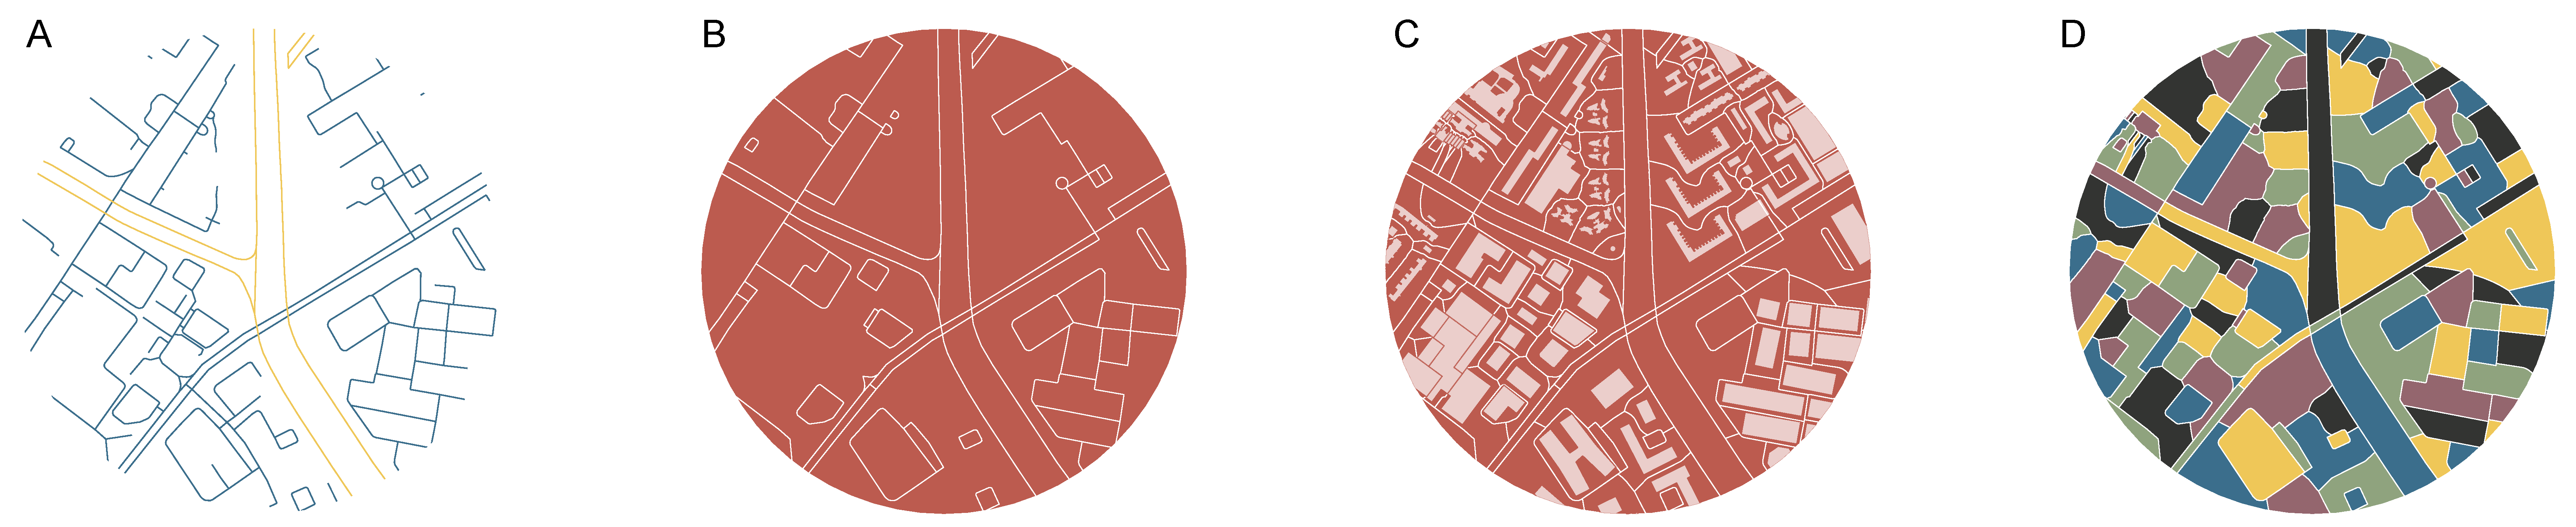
\includegraphics[width=\linewidth]{fig/et_diagram.pdf}
    \caption{Diagram illustrating the sequential steps leading to the delineation of
    enclosed tessellation. From a series of enclosing components, where blue are streets
    and yellow river banks (A), to enclosures (B), incorporation of buildings as anchors
    (C) to final tessellation cells (D).}
    \label{fig:et_diagram}
\end{figure}

Resulting ETCs are indivisible and internally consistent, as they are
linked at maximum to a single building, and exhaustive as they cover the entirety of space
thanks to contiguous geometry of enclosures. Their structure and scale adapts to the
environment and can take a form of a small-scale granular mesh in city centres of
historical origin as well as large-scale polygons encoding the vast natural open spaces.

% - morphometrics
% -- characterisation of building patterns using morphometrics
% -- the principle of inclusiveness (more better) to minimise selection bias
% - context
% -- representation of context as topological distance
% -- reflection of distribution of characters
Having ETCs, building footprints and street networks, we measure a wide range of aspects
of their spatial organisation, from dimensions and shapes of individual objects to their
spatial distribution, intensity or connectivity reflecting configuration of streets. We
call these measurements \textit{morphometric characters}. Since we do not a-priori know
which characters are determining the differences between types of urban
development the most, we aim to include a relatively large set of characters to
avoid potential selection bias, believing that further steps will be able to deal with a
larger amount of input data generated by a larger number of characters\footnote{The list
of measured morphometric characters and their implementation details are available in
the online repository at \url{https://github.com/urbangrammarai/spatial\_signatures}}. As the aim is
to use these characters to detect contiguous homogenous areas of urban form, we are more
interested in tendencies of their distributions within space. Therefore, we link all
values to ETCs and capture the distribution of each within a spatial context
around each ETC. Context here is defined as in terms of topological distance (10 steps)
between ETCs, with each one in reach being weighted by its distance to the original ETC. This
kind of aggregation is adaptive to the pattern of ETCs and reflects the higher importance
of close elements compared to more distant ones.

% - clustering & dissolution
% -- K-Means clustering of ET cells based on morphometric profile
% -- hierarchical approach - sub-dividing interesting clusters via second level K-Means
% -- aggregation of cells into form-based signatures
ETCs characterised by contextualised morphometric characters are grouped using
the K-Means algorithm, effectively deriving a typology of ETCs. Even though K-Means itself does not
contain any contiguity constraint, the design of inherently spatially autocorrelated
characters results in larger clusters that are spatially contiguous. Moreover,
this approach can be potentially applied hierarchically. When further detail
is needed, the algorithm can be run within individual
clusters. Finally, ETCs are
aggregated together based on their class, resulting in the set of spatial
morphosignature geometries, where
each contiguous area assigned the same cluster represents a single morphosignature.

% - case study - GB
We deploy this approach on the case of Great Britain, illustrating both
potential and limits of the analysis of urban form at scale.
% - data
% -- input data in general
% -- input data in the GB
% -- OS Open Map
% --- potential limitation of open data
% -- OS Open Roads
All the datasets we rely on are available openly. First, for
barriers encoding delimiters of enclosures,  we use the following: street
networks from the ``OS Open Roads'' data product,
representing street centrelines; railways from the ``OS
OpenMap - Local''; rivers from ``OS OpenRivers''; and a coastline from OS
Strategi® (REF). All these products are released by the Ordnance Survey under
an Open Government License, allowing us to release the
resulting classification as an open data product. The second input is the layer capturing
building footprints, which is again retrieved from the ``OS OpenMap - Local''. However, the
data reflect aggregated footprints and do not distinguish between individual buildings
when they are adjacent. While that is indeed a limitation, the method is designed and
tested \citep{dab_mf_2021} to be robust enough to accommodate for various
sub-optimal data sources.


\section{Results}
\label{sec:res}

% - 19 classes within 3 groups
The resulting classification of Great Britain identified 19 types of form-based
signatures that can be organised into three macro groups: countryside, suburban low
density development and dense city centres. It is a result of two hierarchical steps
based on K-Means clustering, where the first resulted in 7 classes, of which the two
most urban have been further clustered into 6 and 8 lower-level classes (after a removal
of outlier classes). An illustration of the classification in London is shown on figure
\ref{fig:london} and in Birmingham on figure \ref{fig:bham}.

\begin{figure}
    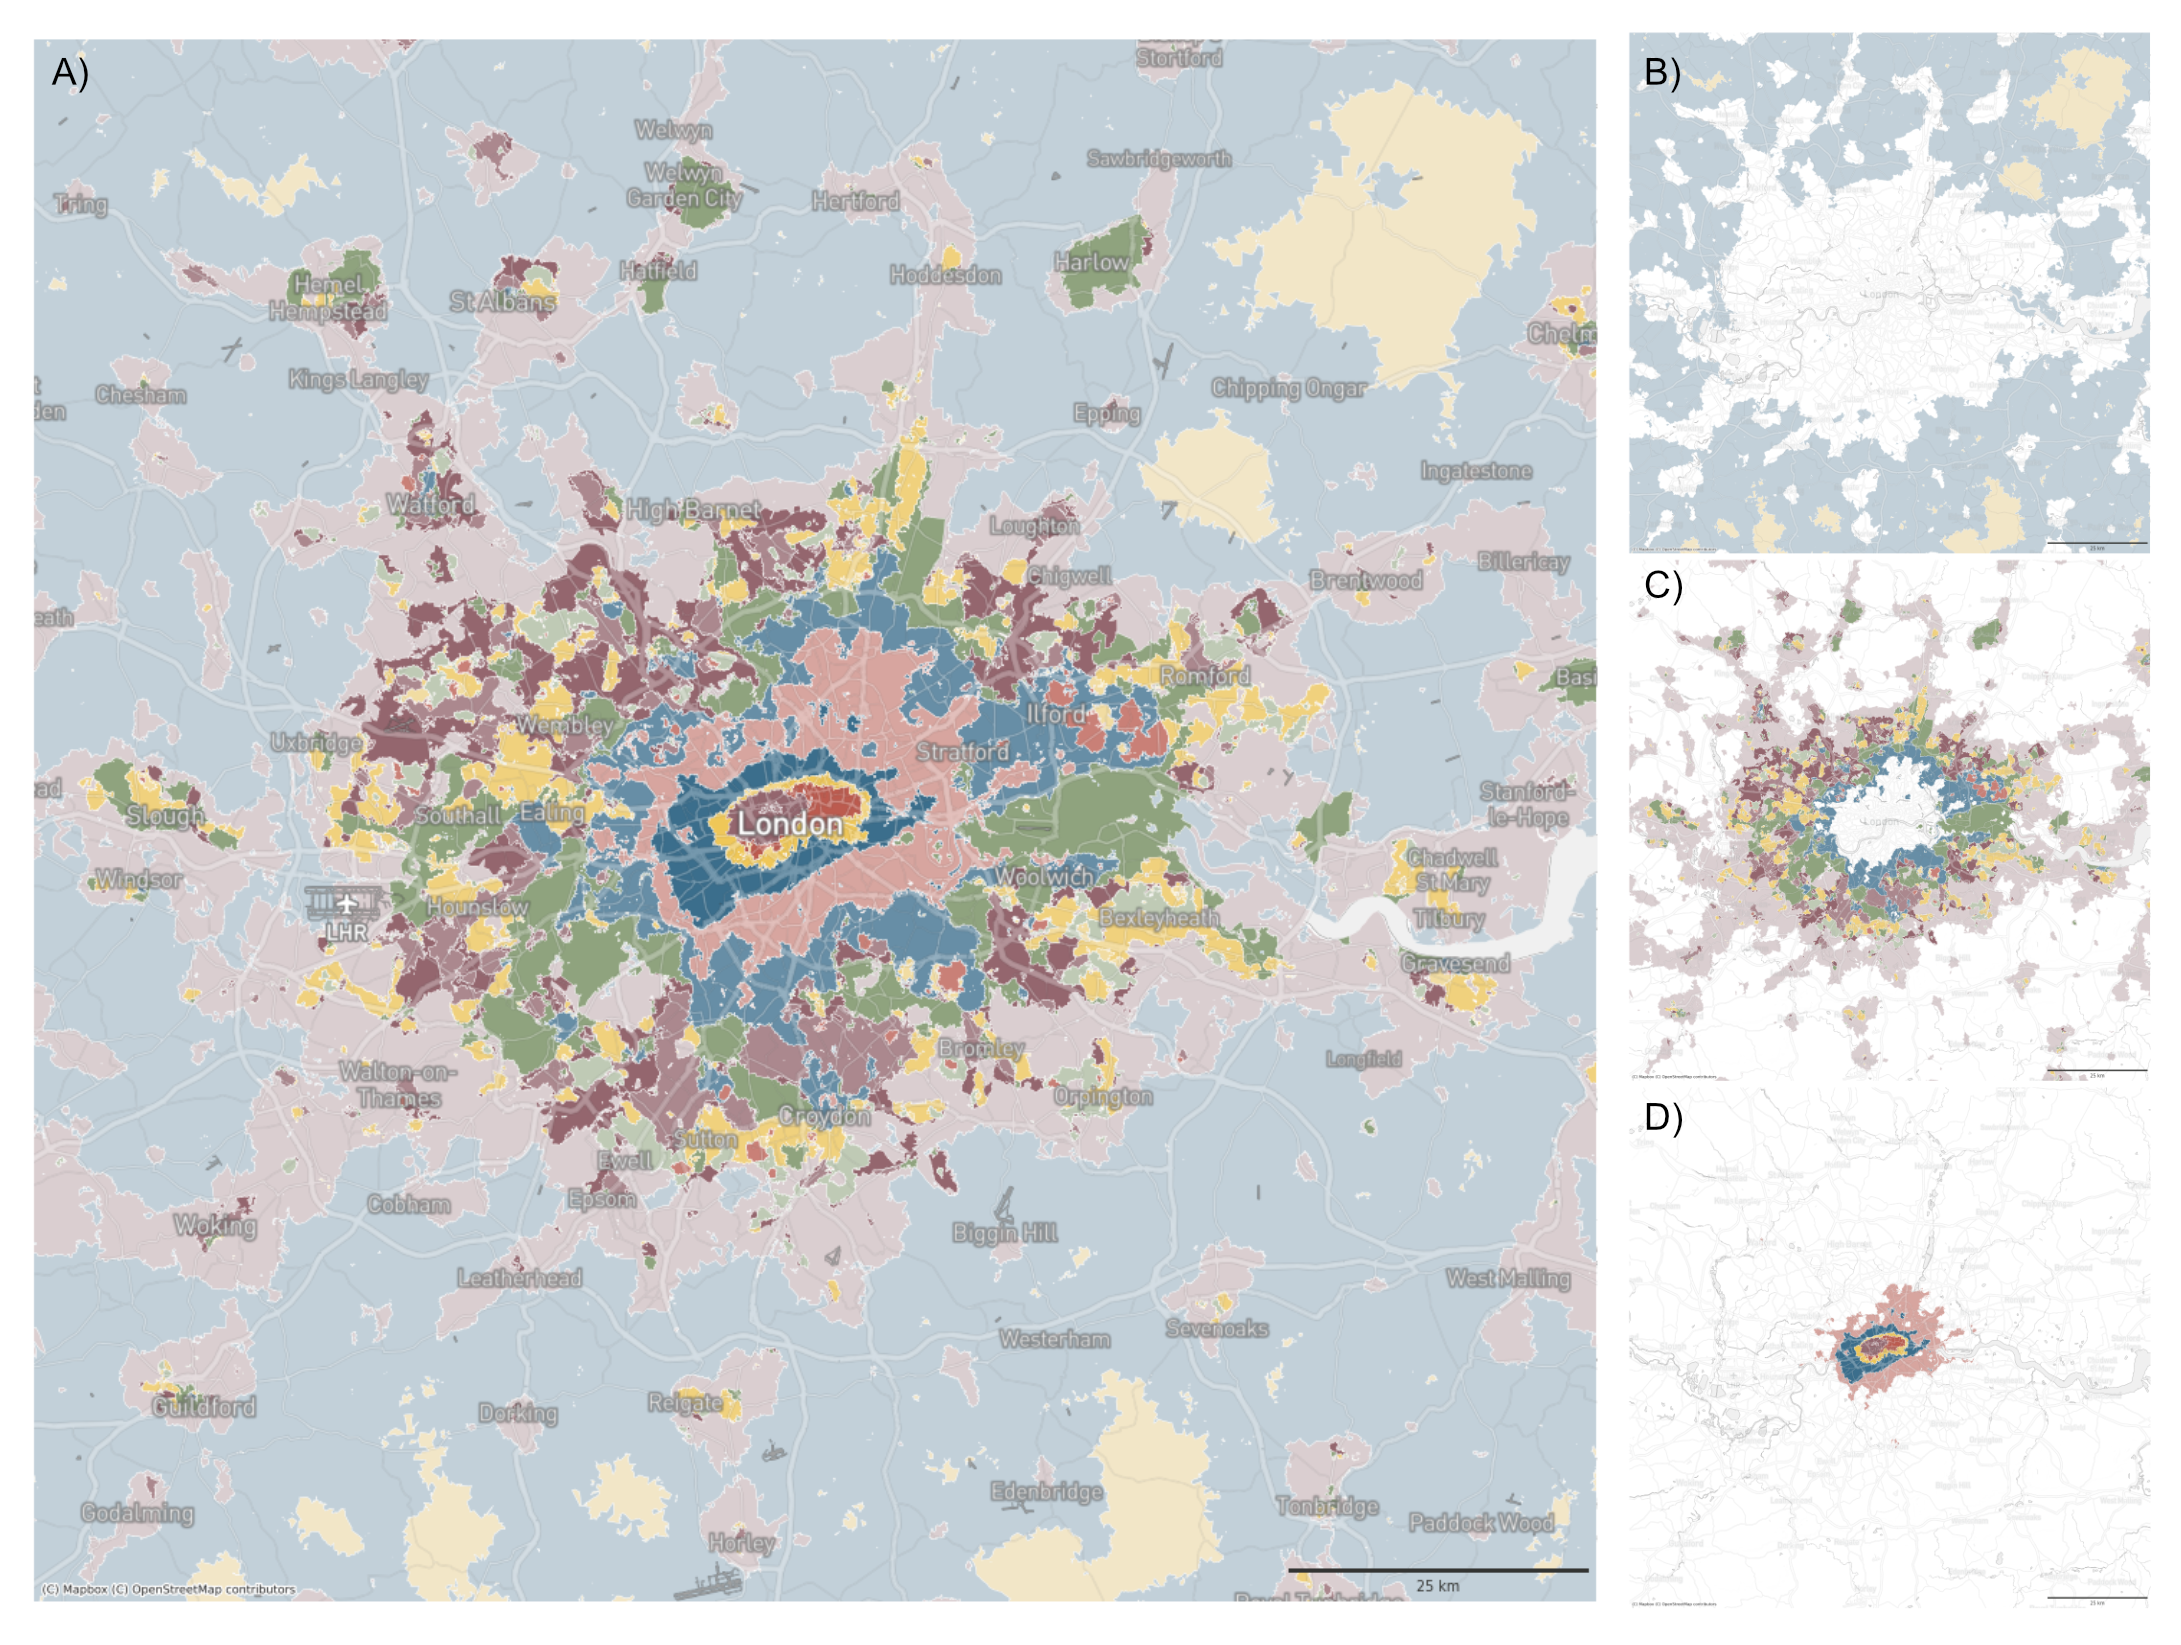
\includegraphics[width=0.75\linewidth, center]{fig/london.png}
    \caption{Form-based spatial signatures in London (A), and their classification into
    top-level macro groups (countryside (B), suburban development (C) and city centres
    (D)).}
    \label{fig:london}
\end{figure}

% -- countryside --- brief portrait
Countryside macro group is composed of four signature types covering large-scale open
spaces from agricultural land in southern England to vast natural areas of Scottish
Highlands. The urban development in this group is limited to small villages or hamlets.
All four classes are a result of the first clustering step.

\begin{figure}
    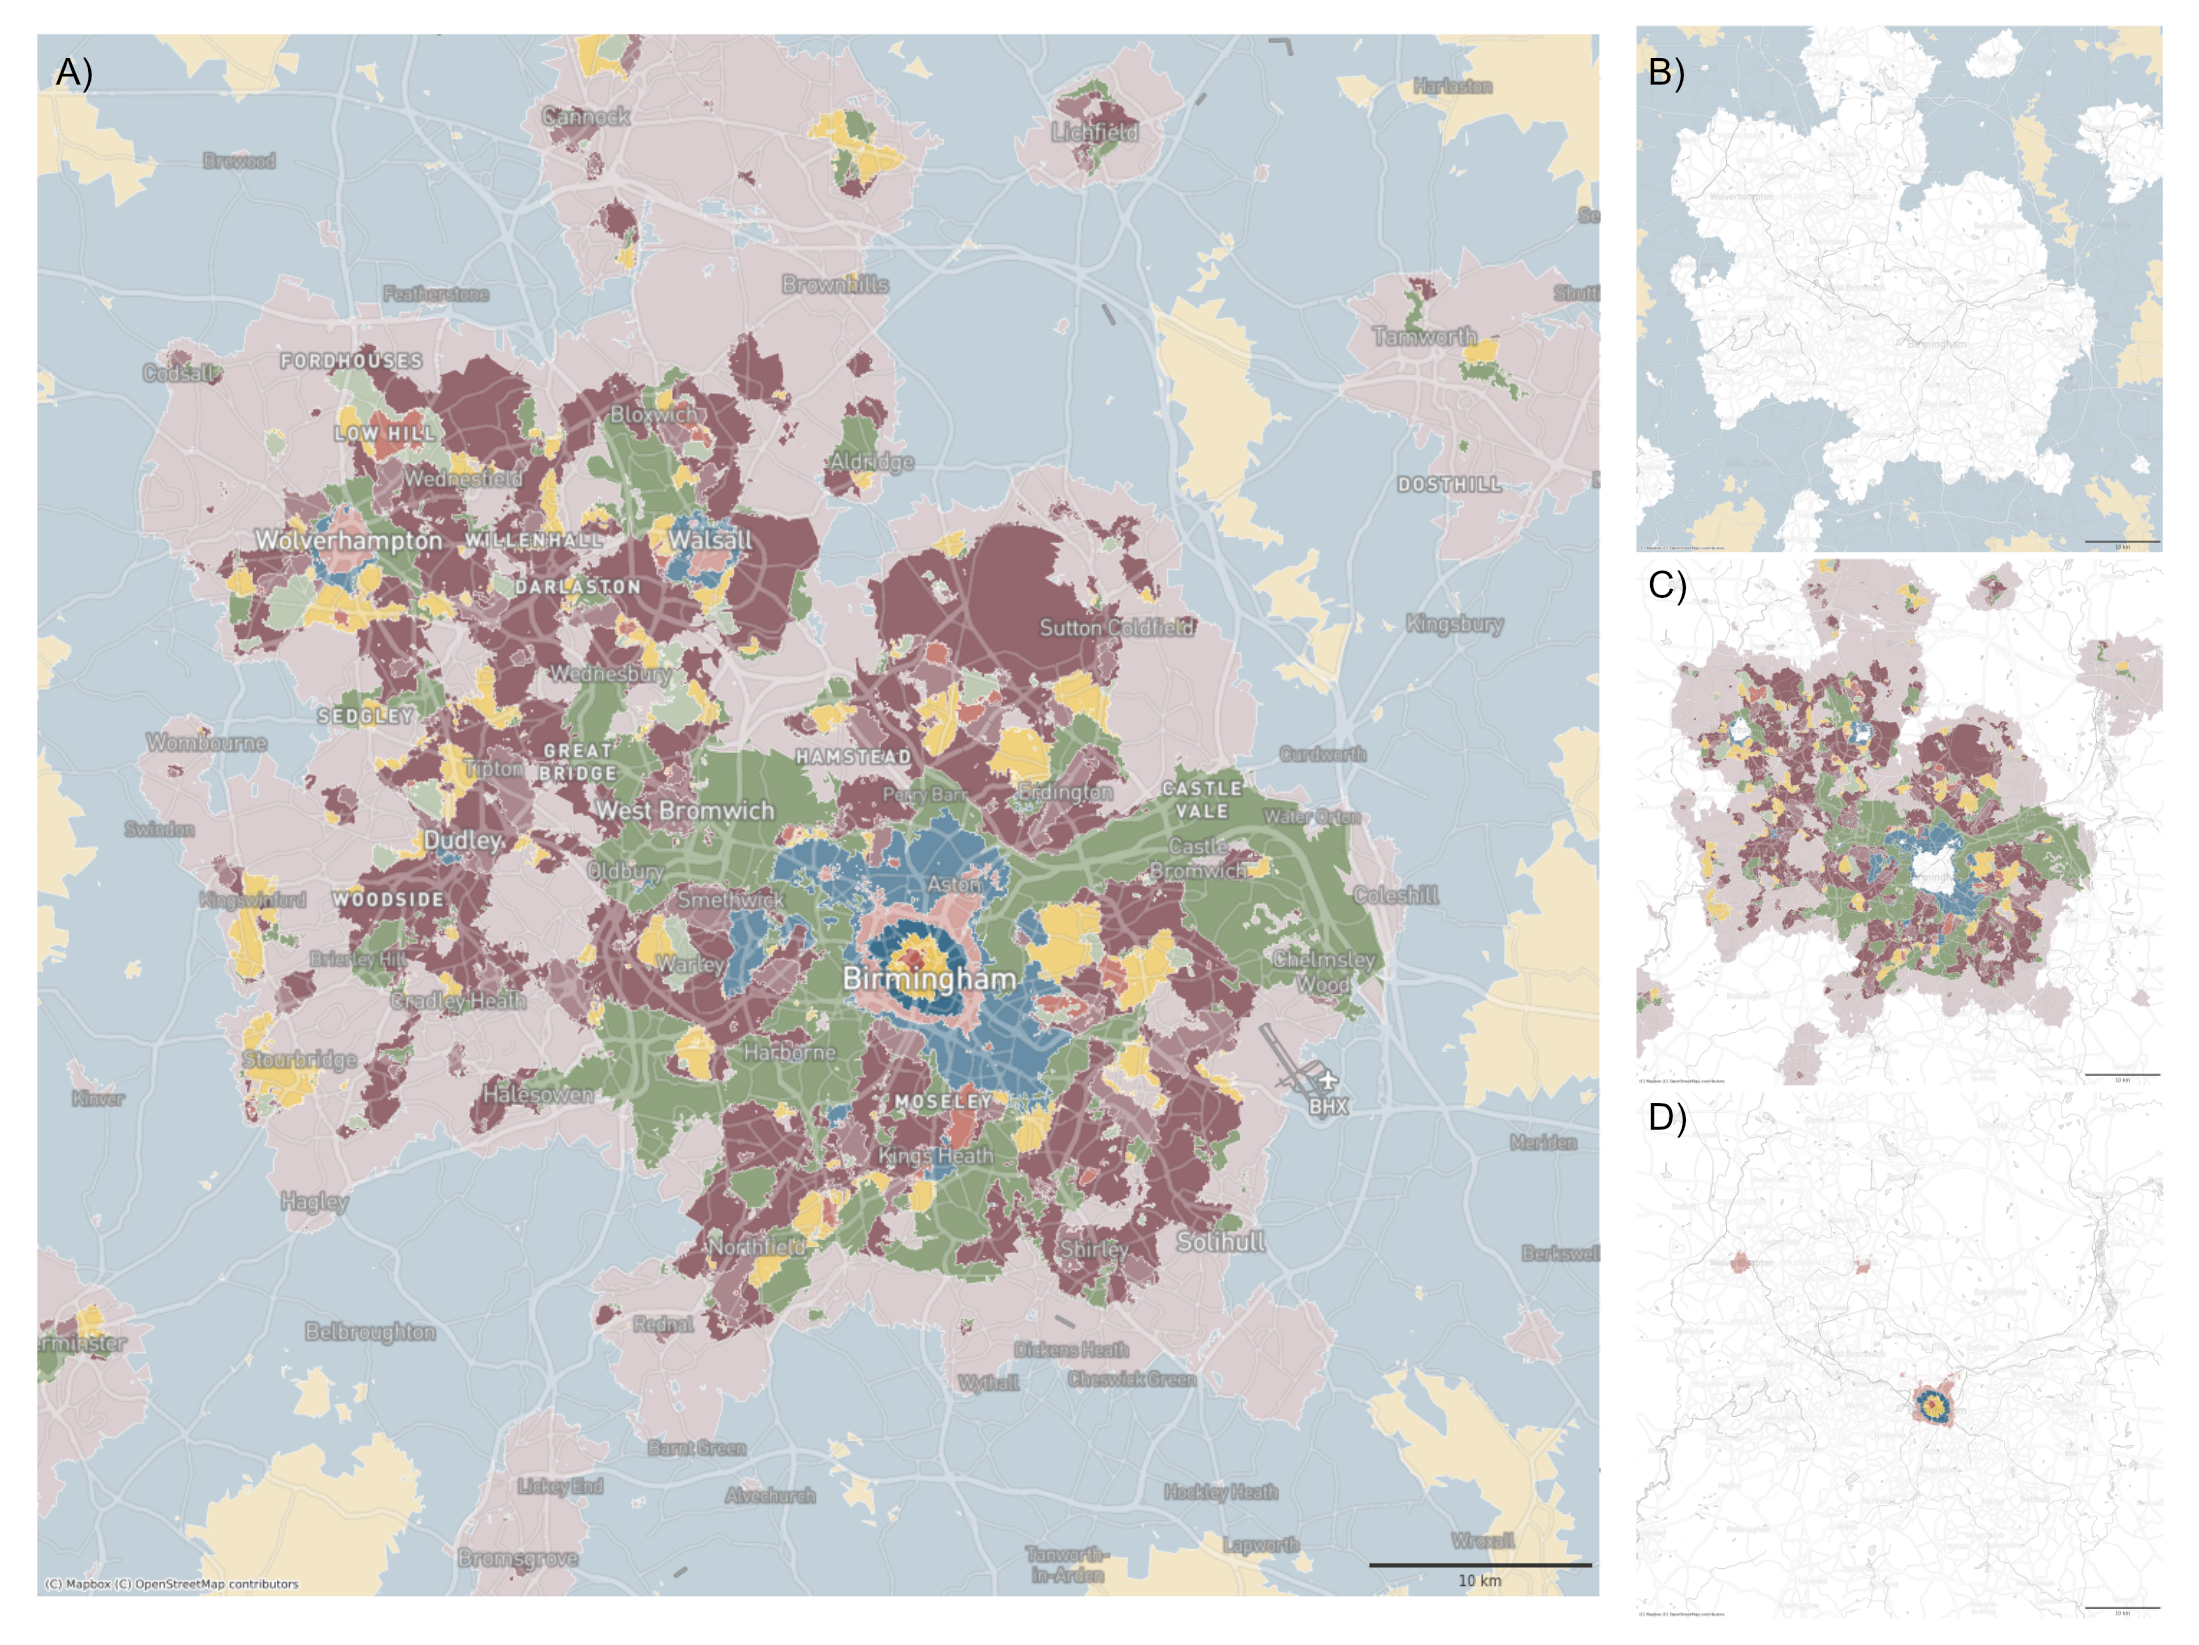
\includegraphics[width=0.75\linewidth, center]{fig/bham.png}
    \caption{Form-based spatial signatures in Birmingham (A), and their classification
    into top-level macro groups (countryside (B), suburban development (C) and city
    centres (D)).}
    \label{fig:bham}
\end{figure}

% -- suburbs --- brief portrait
Second macro group covers suburban low-density development areas, taking up most of the
area of british cities. We can identify 9 types of signatures, originating in two
classes from the first step. The range of types stretches from sparse single-family
housing on the peripheries of cities, planned residential developments of 20th century
to predominantly industrial areas. The types differ in many aspects, from the overall
built-up density and related geometry of both enclosed tessellation and enclosures (both
affecting the description via many morphometric characters) to connectivity of street
networks or their solar orientation.


% -- city centres --- brief portrait
Final macro group comprises of dense town and city centres, all originating from the
single top level cluster. These signatures reflect the main hubs of activities in each
larger settlement. In some cases, they are all located in the same central areas, while
in others some local district nodes show up (e.g. Liverpool). All six types can be
arranged according to their level of \textit{urbanity} and tend to form concentric
rings.


% - Concentric character of British centers and centre hierarchy -- from London to
%   Oxford
Two types are exclusive to London's city centre (roughly around Soho as show on figure
\ref{fig:centres}A) and are not present anywhere else in the whole country. The
remaining are present in other places and their presence can encode the
\textit{urbanity} of each city or town. For example, Birmingham as the second largest
city in the country contains four types of central signatures (figure
\ref{fig:centres}B), compared to six in London. Scottish capital Edinburgh contains only
three (like many other cities across the country (e.g. Manchester or Glasgow))
illustrated on figure \ref{fig:centres}C. Smaller cities like Southampton have only two
types (figure \ref{fig:centres}D) and towns as Oxford are limited to a single central
type (figure \ref{fig:centres}E). The presence of types is not accidental -- smaller
cities lack the most urban types, while all of them contain the least urban type.

\begin{figure}
    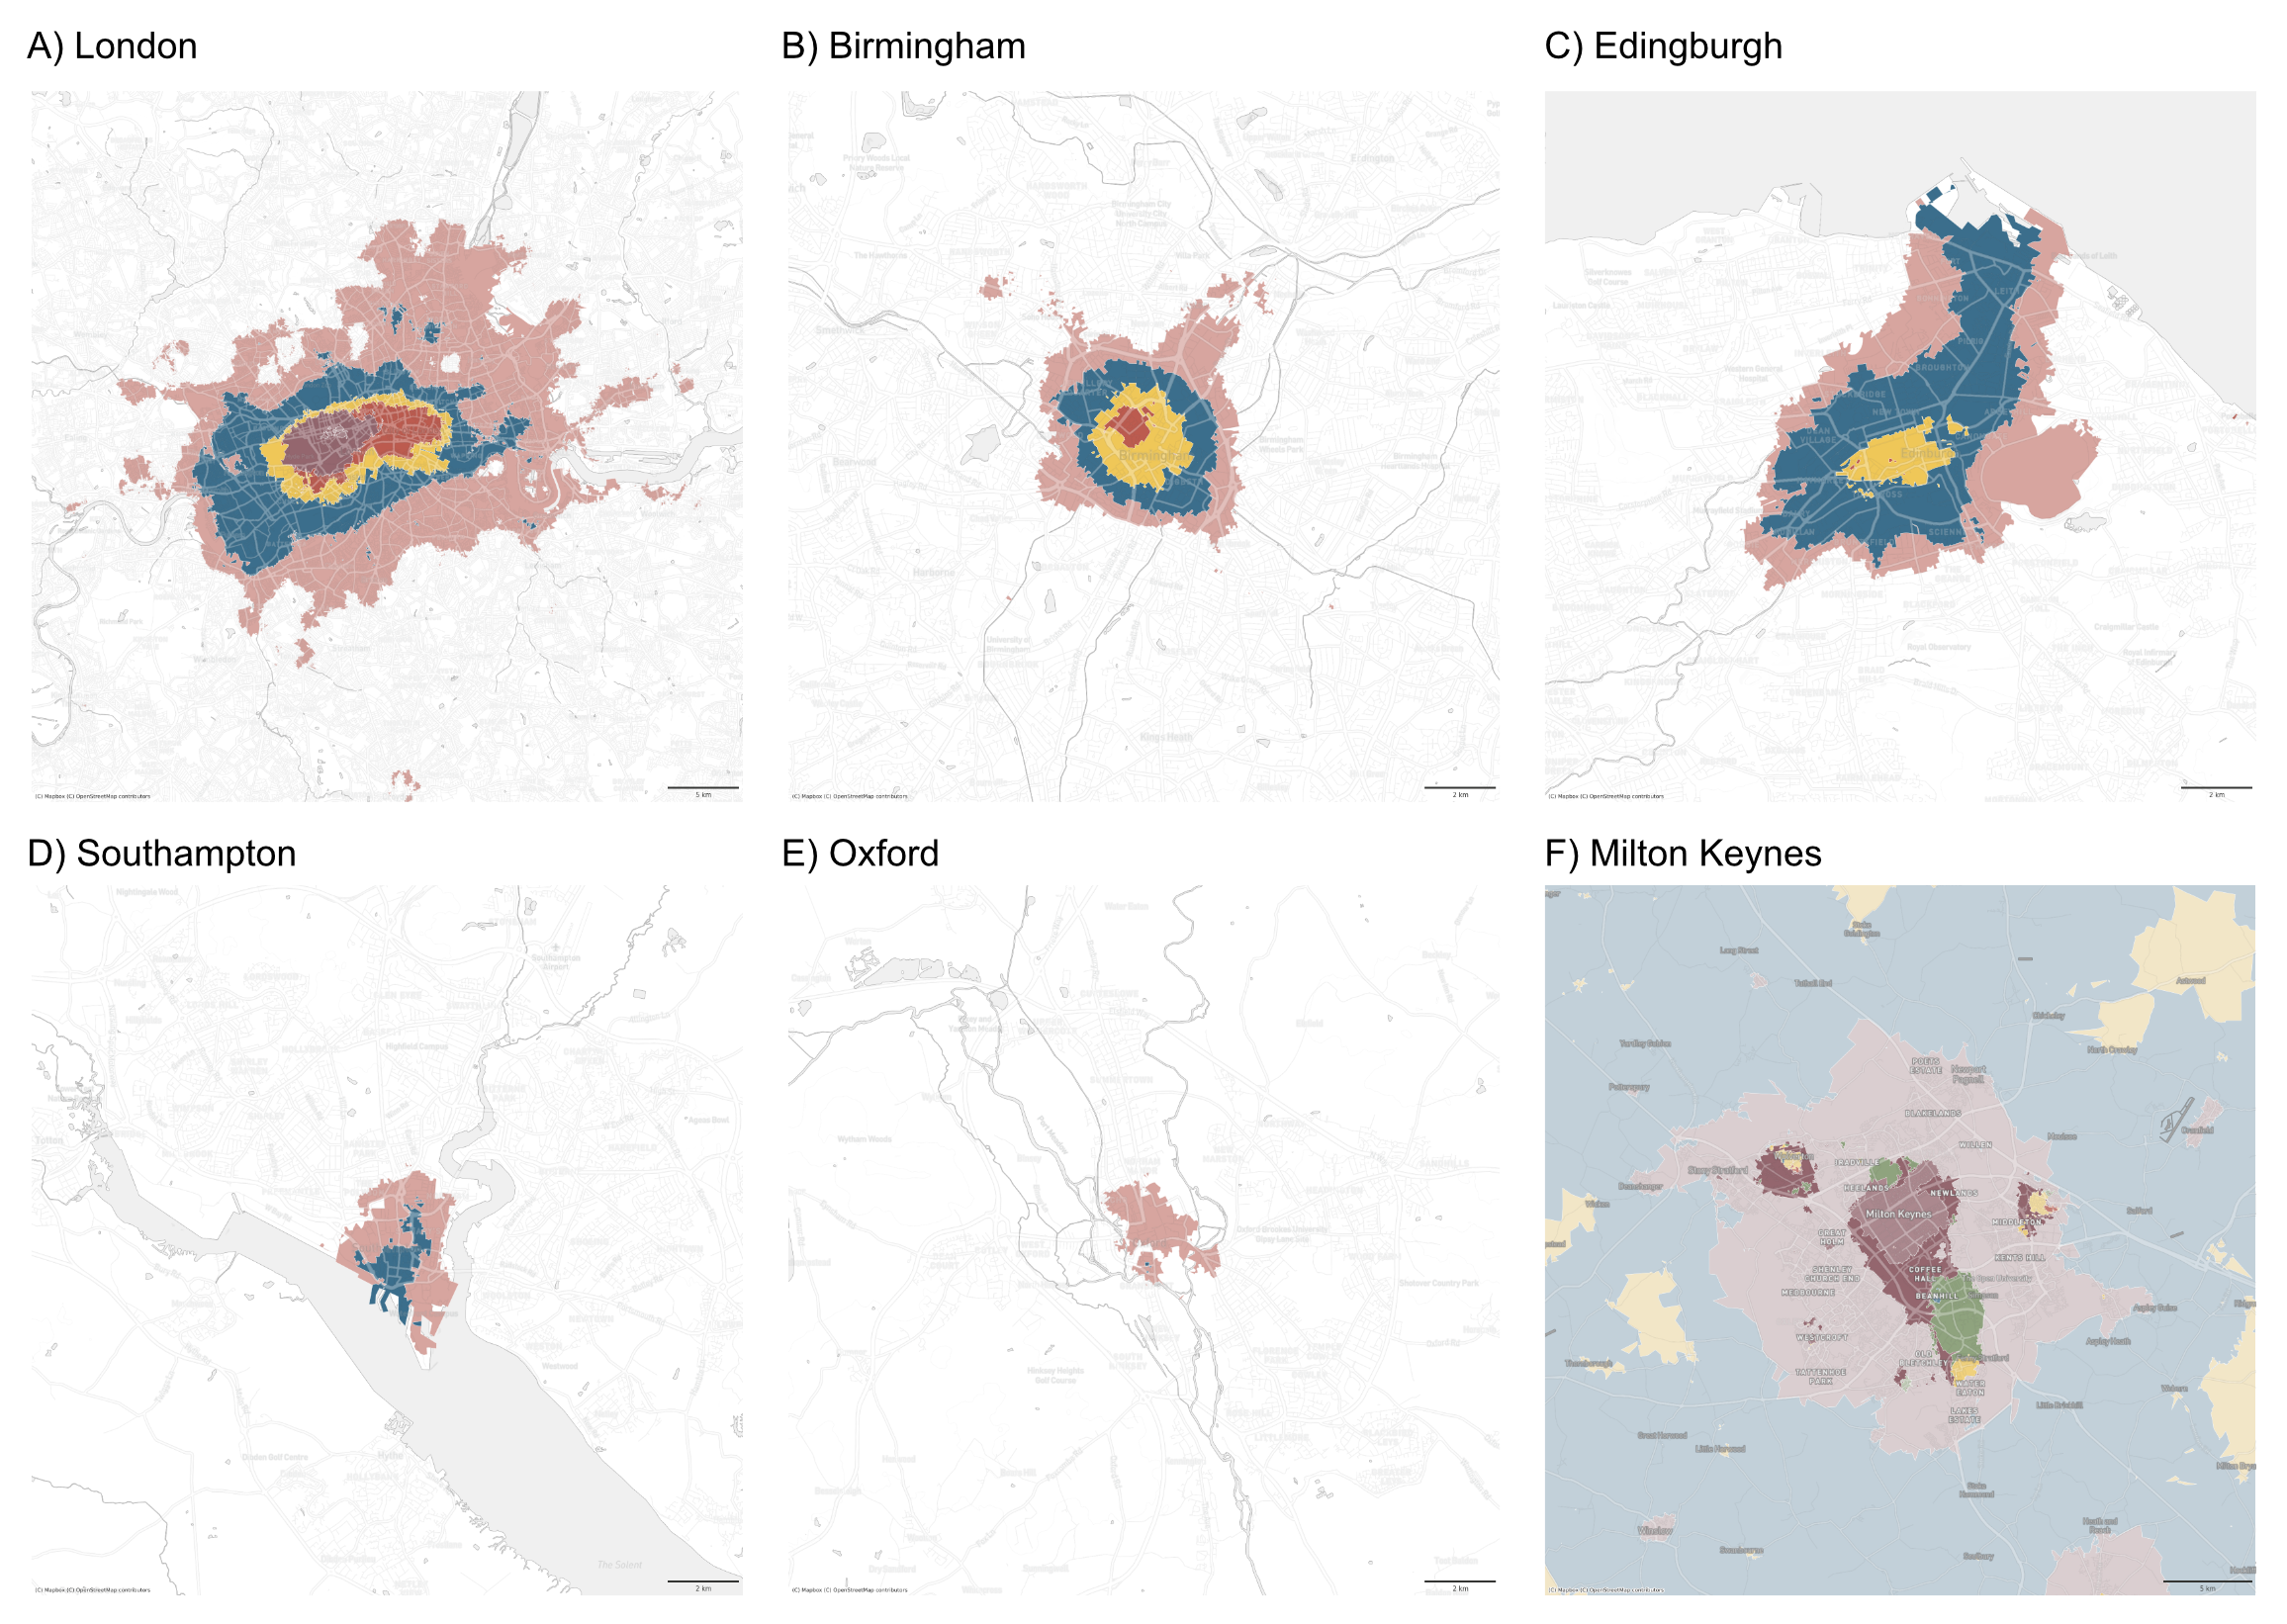
\includegraphics[width=0.75\linewidth, center]{fig/centres.png}
    \caption{Hierarchy of city centres from the most urban with all six signature types
    belonging to city centres macro class in London (A), four types in Birmingham (B),
    three in Edinburgh (C), two in Southampton (D) and one in Oxford (E). Milton Keynes
    (F) does not have an area classified as morphological centre.}
    \label{fig:centres}
\end{figure}

% -- Milton Keynes does not have a morphological centre
Notable is the case of Milton Keynes, a new town built since 1960s on the green field
with a target population of 250 000 (currently at 230 000). Its development followed a
carefully designed masterplan, laying out the whole city. However, the resulting
structure is very different from any other city in the country as none of the signatures
encoding urban centre is not present in Milton Keynes. We could say, that it does not,
have a morphologic centre, as illustrated on the figure \ref{fig:centres}F.


\section{Discussion}
\label{sec:disc}

% - signatures in the context of morphological studies
% -- conceptual similarity with morphological region, urban tissue and similar
% -- differences between the concepts and resulting complimentarity
    % different scales, different purposes, different questions
The spatial signatures framework, either based on a combination form and function or a
single component, aims to identify and delineate recurring patterns of urban
spaces. As
such, it is deeply embedded in the tradition of urban morphology, directly related to
established concepts like morphological region, urban tissue and similar. All
of them aim to
determine which areas of cities are internally consistent. The differences
between these perspectives stem from the methods they rely on, which
undoubtedly results in variation in the classifications of urban form they
produce. Where
historico-geographical morphological region would detect the original development and its later
expansion following a similar pattern as two distinct areas (due to a different
historical origin), the morphosignatures would class them in a single area as the pattern
is homogenous. Which of the two is the \textit{correct} answer then fundamentally
depends on the question asked. Each of the concepts and related methods of their
analysis are bound to different scales, purposes and questions, and are complimentary
rather than competing.


% - reproducibility of morphological studies
% -- morphometric methods can be algorithmised, hence easily replicable and reproducible
Unlike traditional urban morphology that is based mostly on qualitative methods requiring 
 expert knowledge and interpretation, morphometric studies offer a high
degree of reproducibility and scalability. Methods are often embedded in
computer code release under open licenses which, given the same input data,
produces the same results. This reliability of the method is especially
important in the policy-making context which needs to be consistent across years and
updates of supporting morphological data.

% - limits
% -- in the context of morphometrics
% --- suboptimal data input (individual buildings)
%   --- national extent and hence resolution of clustering - local differences may be
%   smoothed out as insignificant from the national perspective
% --- precision of boundary placement

Morphometric approaches have their limitations, related to the the dependency on the
quality of input data as well as the behaviour of used algorithms. Suboptimal
input data can significantly affect the performance of morphosignature detection. Take, for example,
the quality of building footprints as one of the most utilised data source. While there
is a wide range of reliable, mostly governmental or municipal, sources of data
for some regions of the world, this is not the case everywhere. Some sources, like OpenStreetMap, provide highly
inconsistent data, with some buildings drawn in high detail and others in very
coarse ways. Fortunately, technology is moving very rapidly and advances in
data collection and creation (e.g. building footprints derived from satellite
imagery) may change this landscape for the better in the coming years.

The algorithms used to classify features into morphosignatures also make a
difference, as does the scale at which an analysis is run.
Our classification and, to a degree, the
\textit{resolution} at which the clustering is done is national. This choice may result in local
differences being smoothed out if they are less relevant from the national
perspective. Zooming into individual neighbourhoods, one may find some of the
decisions made by the algorithm too coarse. The same applies to the placement of the boundaries between morphosignatures.
The trained urban morphologist or urban designer might question why one building
belongs to a type A, while the other one within the same block is assigned to
type B. It is important to
keep in mind the scale and goal of the classification, which is then embedded
in the algorithmic choices.

% - scalability of morphological studies
% -- we can ask questions about larger patterns that we did before
% -- we can look into cross-national similarities and tendencies
Our main contribution with respect to traditional
morphological studies resides in the scalability of the analysis. With national-scale data we can ask
fundamentally new questions about the emergin patterns than is possible with
smaller scales. Obtaining the analysis covering
the same extent as the one just presented at the same level of detail using
historico-geographical or typo-morphological methods would be simply an unfeasible task.
Morphometrics allows us to begin considering cross-national comparisons that
consider detail at neighbourhood-like scale.
%
As we develop more fine grained and scalable classifications, an
important challenge will be to devise ways that allow us to blend the
insights we can gain at this scale with the body of knowledge developed over
time from more qualitative approaches.

\section{Data and code availability}
The repository, containing reproducible code in Jupyter notebooks is available at
\url{https://urbangrammarai.github.io}. Guidelines on how to access and
download the resulting classification are available in the same website.


\clearpage




\bibliographystyle{apalike}
\bibliography{refs}

\clearpage

\end{document}
